

\section{Expedition Overview}

Twenty-two expedition members travelled from the UK for a total of 65
person-weeks in the field, with 88 person-trips in our callout roster.
Seventeen from the UK stayed at underground camp, along with six
Slovenes from the local JSPDT club, a total of 95 people-nights at camp.
All successful exploration took place on camping trips.

This was the first expedition for three first-year UK students, all of
whom stayed at underground camp and discovered significant quantities of
new cave.

In all, the cave consumed a kilometre of rope for the rerigging of the
main pitch series, and newly explored sections left rigged (or with rope
pulled up) for 2011.

In terms of establishing the connection between \emph{Vrtnarija} and
System Migovec, no work during the 2010 expedition went into \emph{M2}
(\emph{Kavkna Jama}). However, during the early Autumn two JSPDT trips
capped through the tight rift at the very end of the cave
(\textasciitilde -390 m), discovering and then descending a
\textasciitilde 60 m pitch.

The prospects for exploration in 2011 are extremely good.

The extensive horizontal development has led to the discovery and
initial exploration of a number of independent streamways and associated
pitch series, in a horizontal slice of the mountain we have never
visited. Camp \emph{X-Ray} is well suited for the continual exploration
of these leads. We therefore left the camp partially equipped (roll
mats, tent, a small quantity of sealed gas cylinders and fuel).

\begin{figure*}
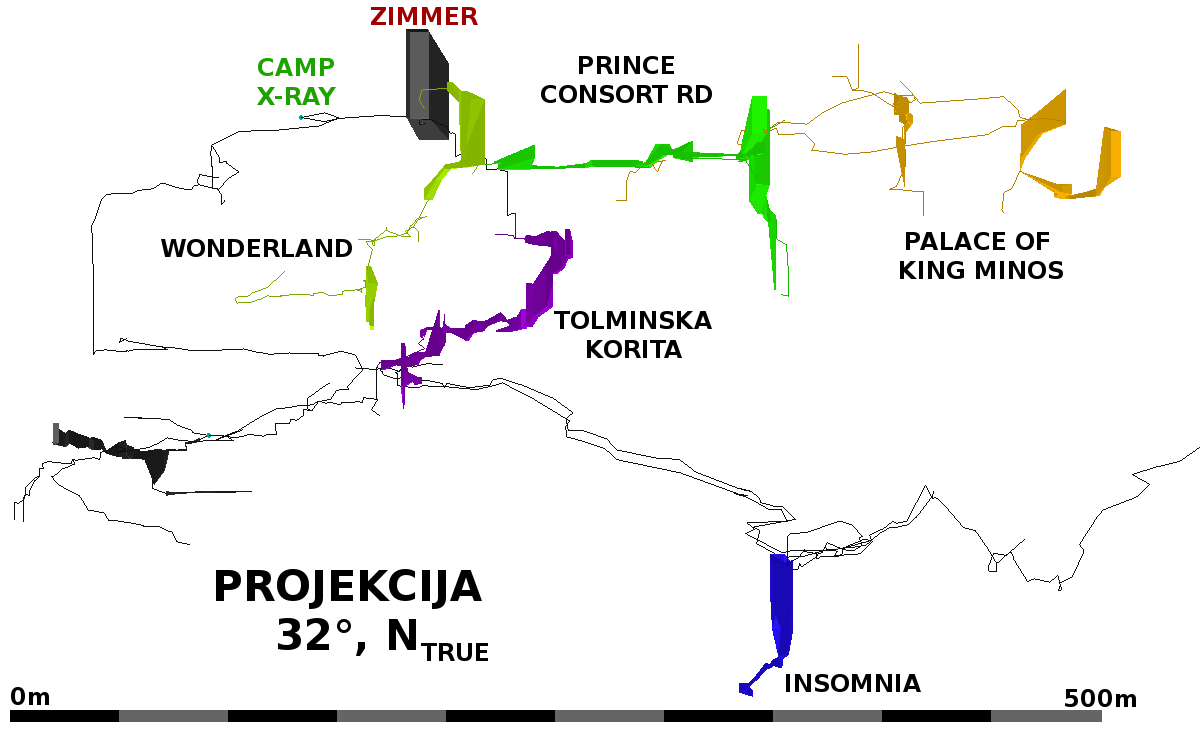
\includegraphics[width=0.85\columnwidth]{2010/overview/2010_deep_vrtnarija_colour_coded_inverted_labelled.png}
\caption{Colour coded diagram of new cave discovered \& surveyed in 2010 in
Vrtnarija.}
\end{figure*}
